\documentclass{beamer}
\usetheme{Hannover}
\usecolortheme{dolphin}

\usepackage[T1]{fontenc}
\usepackage[utf8]{inputenc}
\usepackage{upgreek}
\usepackage{polski}
\usepackage[polish]{babel}

\usepackage{listings}
% \usepackage{array}
% \usepackage{amsmath}
% \usepackage{mathtools}
% \usepackage{caption}
% \usepackage{tocloft}
% \usepackage{tabularx}
% \usepackage{xcolor,colortbl}
% \usepackage{hhline}
% \usepackage{wrapfig}
% \usepackage{enumitem}
 \usepackage{graphicx}
 \usepackage{tikz}
% \usepackage{titlesec}
% \usepackage{subfig}
% \usepackage{pdflscape}
% \usepackage{qtree}
% \usepackage{hyperref}

\graphicspath{ {assets/} }

\author[Antoni M. \\ Maciej M.]{
	Antoni Mleczko \\
	Maciej Mionskowski
}

\title[Origami]{Interaktywna wizualizacja instrukcji składania Origami z elementami symulacji fizyki papieru}

\titlegraphic{
\includegraphics[width=0.2\linewidth]{preamble/agh.jpg}}

\date{2020/2021}

\institute{Wydział Informatyki, Elektroniki i Telekomunikacji}

\begin{document}

\begin{frame}
  \titlepage
\end{frame}

\begin{frame}
  \frametitle{Agenda}
  \tableofcontents
\end{frame}

\section{Opis dziedziny}
\begin{frame}
  \frametitle{Opis dziedziny}
  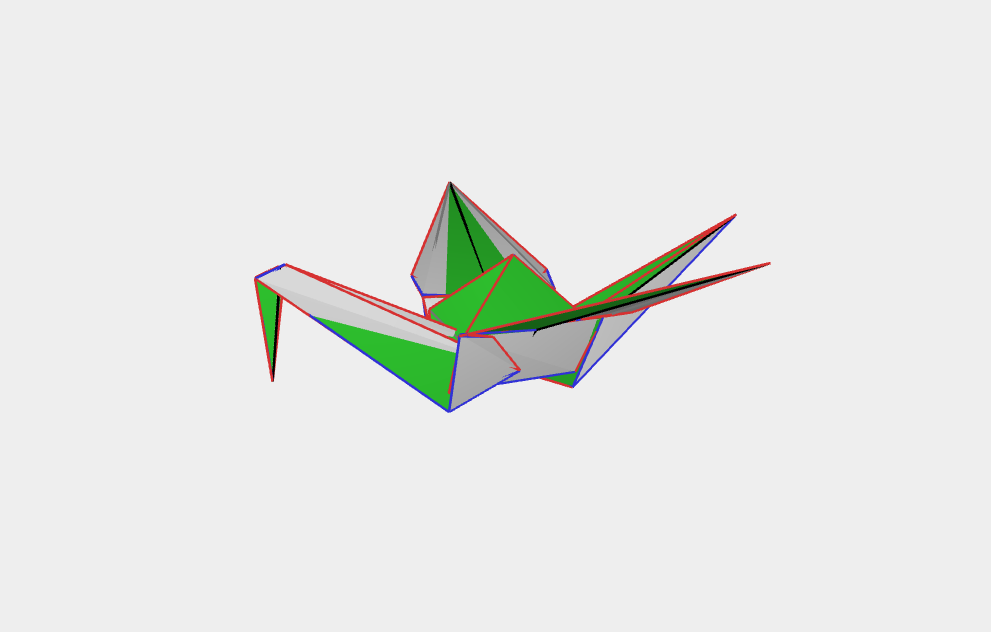
\includegraphics[width=\linewidth]{assets/pres-crane.png}
\end{frame}
\begin{frame}
  \frametitle{Opis dziedziny}
  \centering
	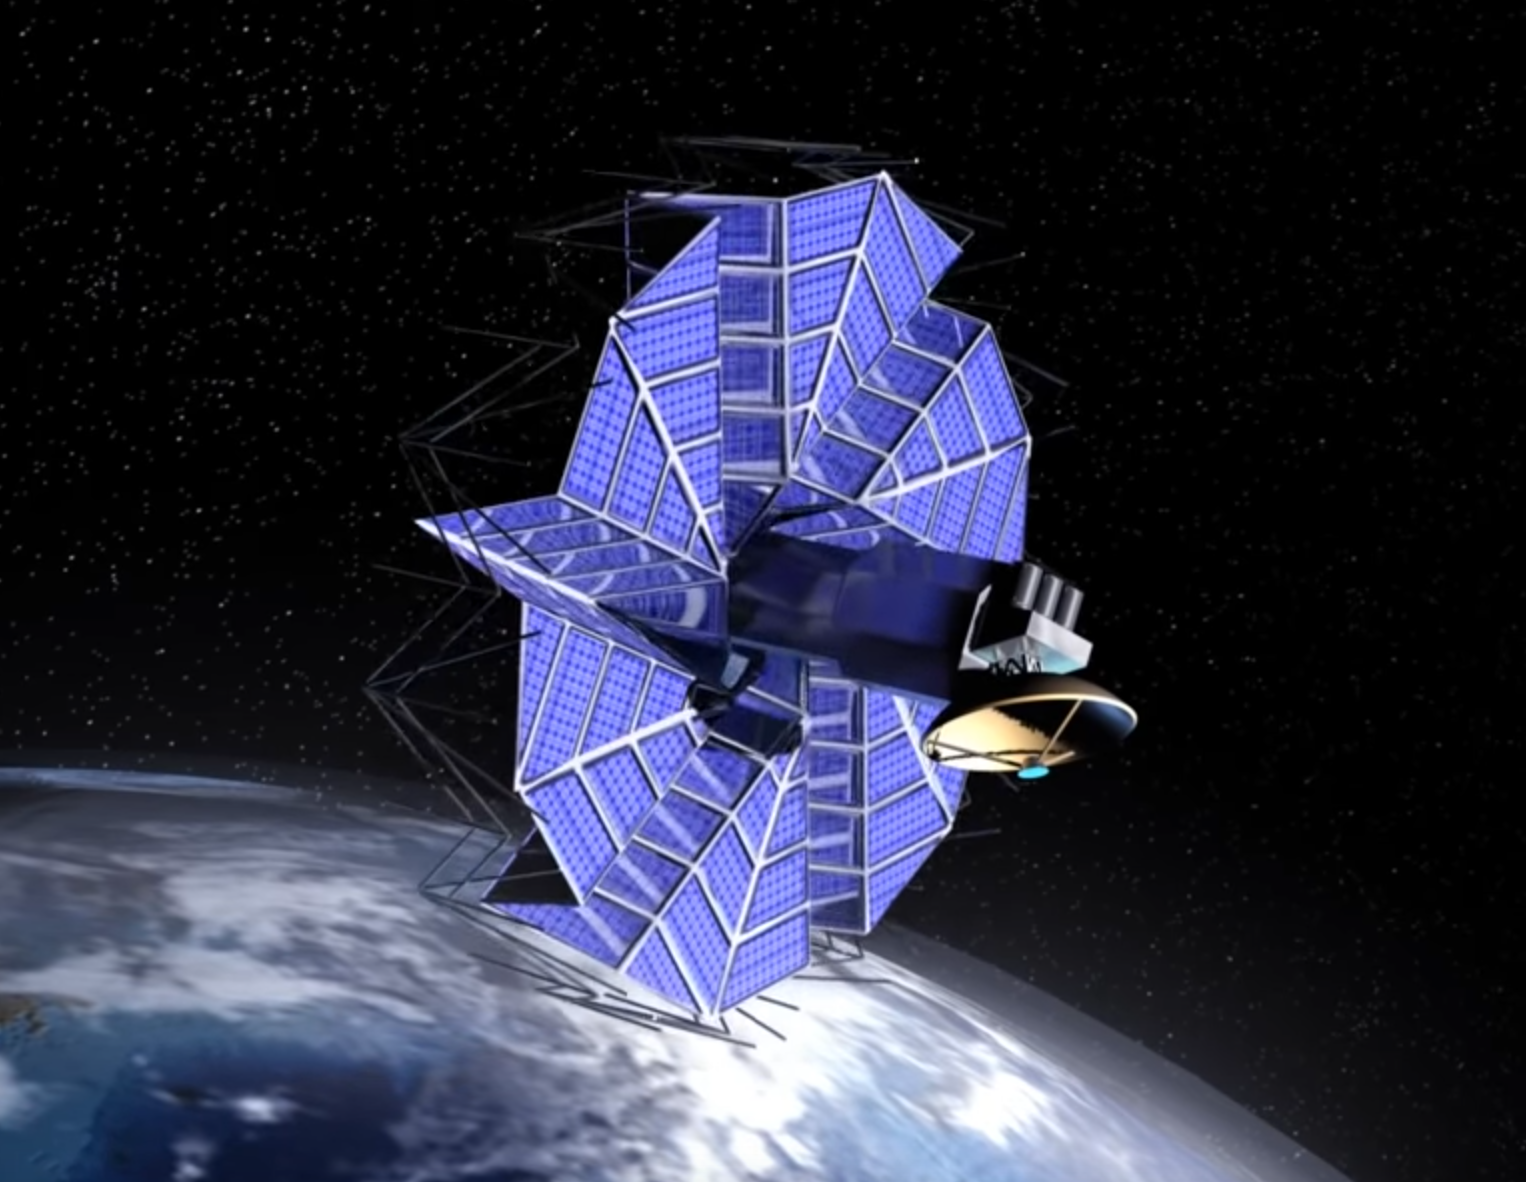
\includegraphics[width=0.9\linewidth]{assets/solar-deployment.png} \\
	\begin{flushright}
		\tiny{Credit: Brigham Young University}
	\end{flushright}
\end{frame}
\begin{frame}
  \frametitle{Opis dziedziny}
	  \centering
	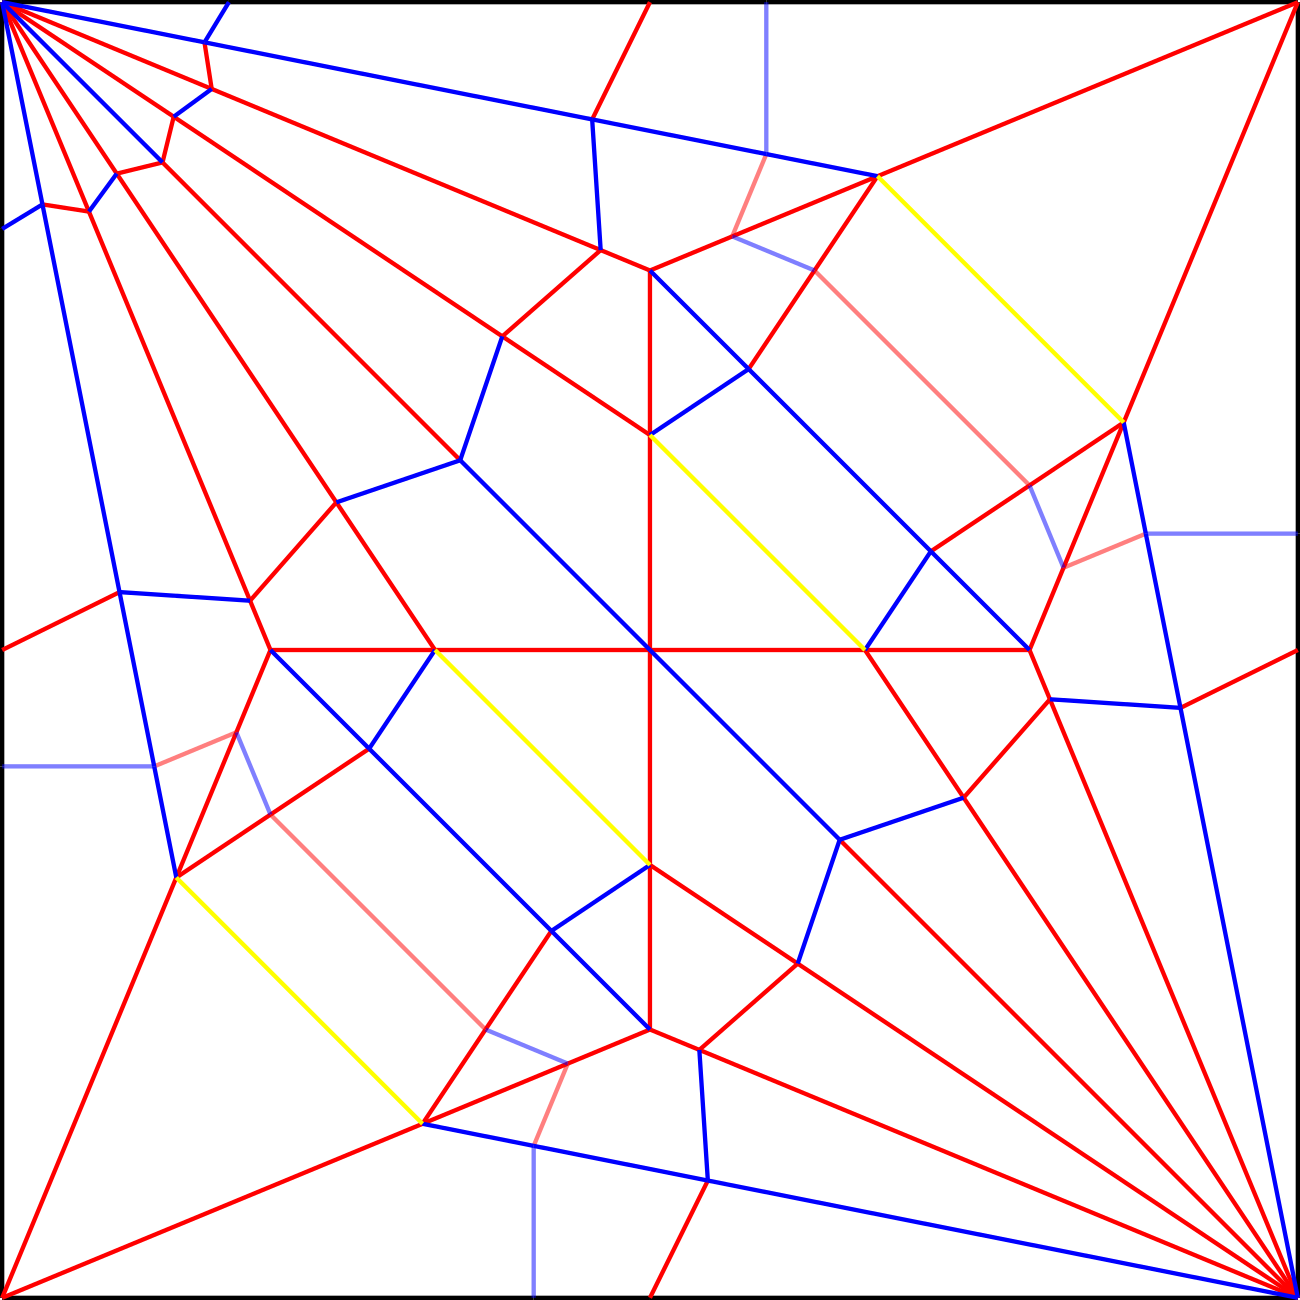
\includegraphics[width=0.7\linewidth]{assets/crane-crease-pattern.png}
\end{frame}

\section{Koncepcja rozwiązania}
\begin{frame}
  \frametitle{Koncepcja rozwiązania}
  \begin{itemize}
	  \item Interaktywna wizualizacja instrukcji
	  \item Format do zapisu złożeń
	  \item Aspekt społecznościowy
  \end{itemize}
\end{frame}

\begin{frame}
  \frametitle{Koncepcja rozwiązania}
	\centering
	  \Huge{Projekt badawczy}
	  \\
	  \small{(prawie)}
\end{frame}

\section{Prezentacja produktu}
\begin{frame}
  \frametitle{Interaktywna wizualizacja instrukcji}
  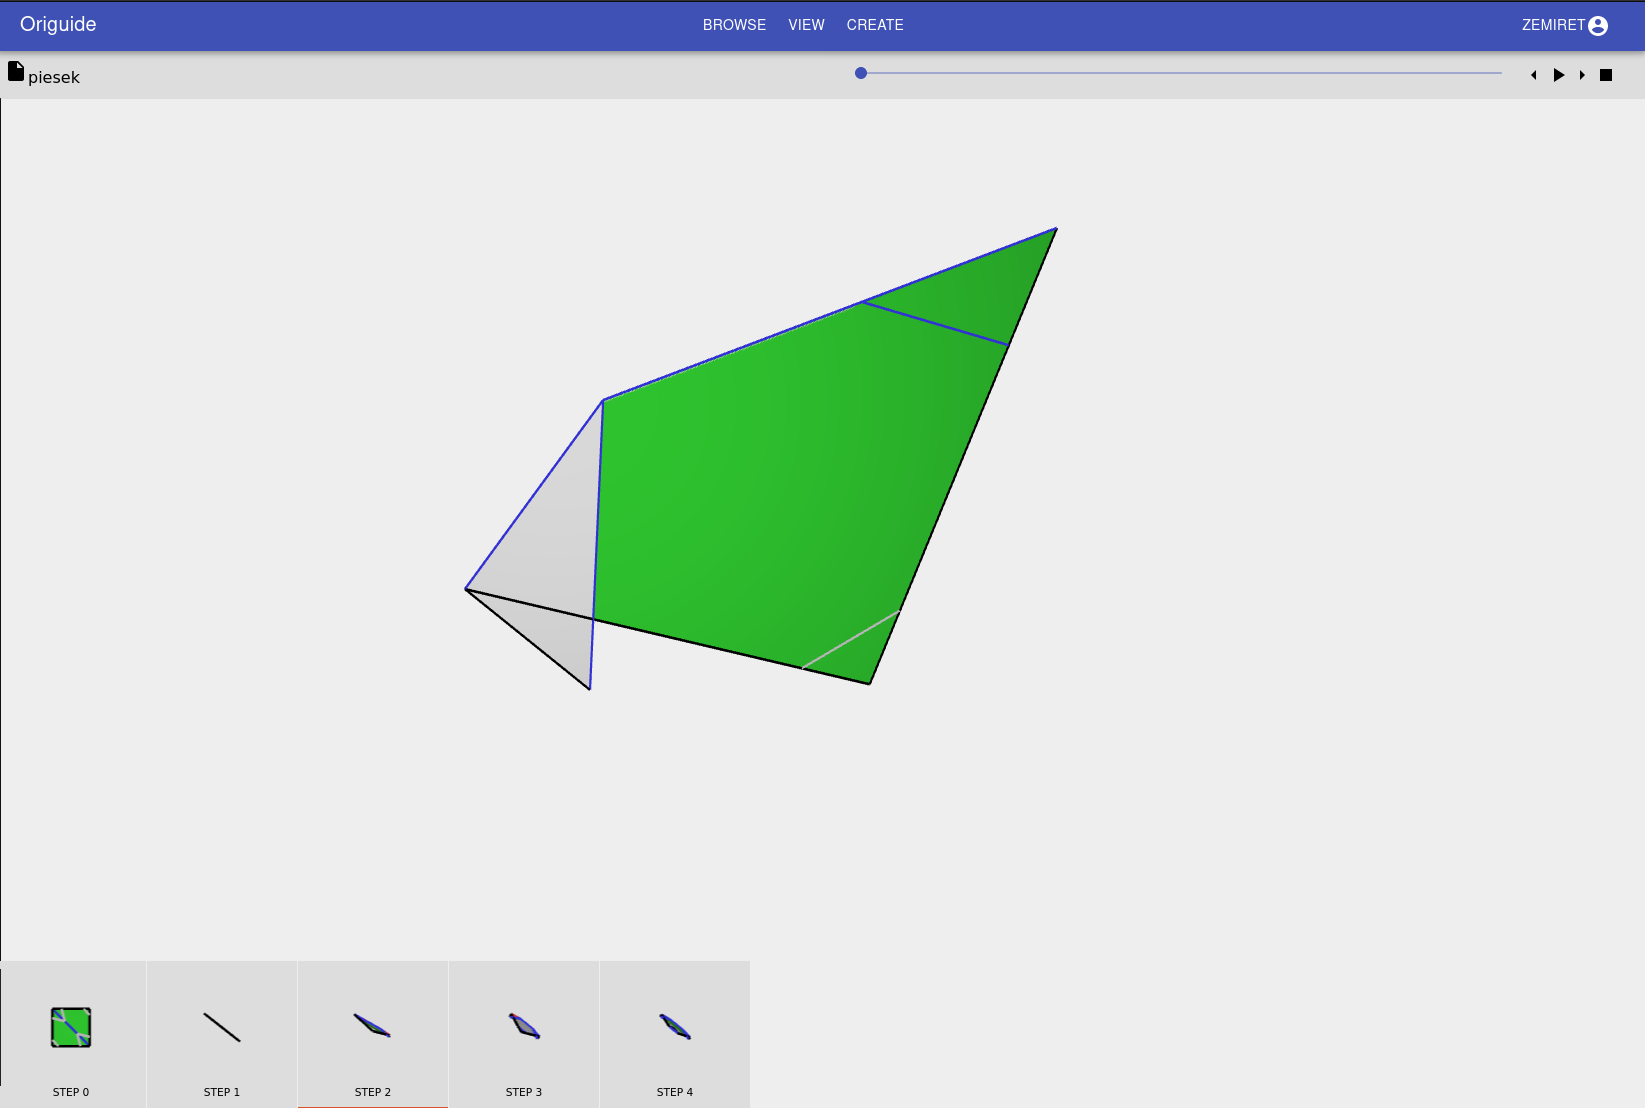
\includegraphics[width=\linewidth]{assets/5-folderView.png}
\end{frame}
\begin{frame}
  \frametitle{Format do zapisu złożeń}
  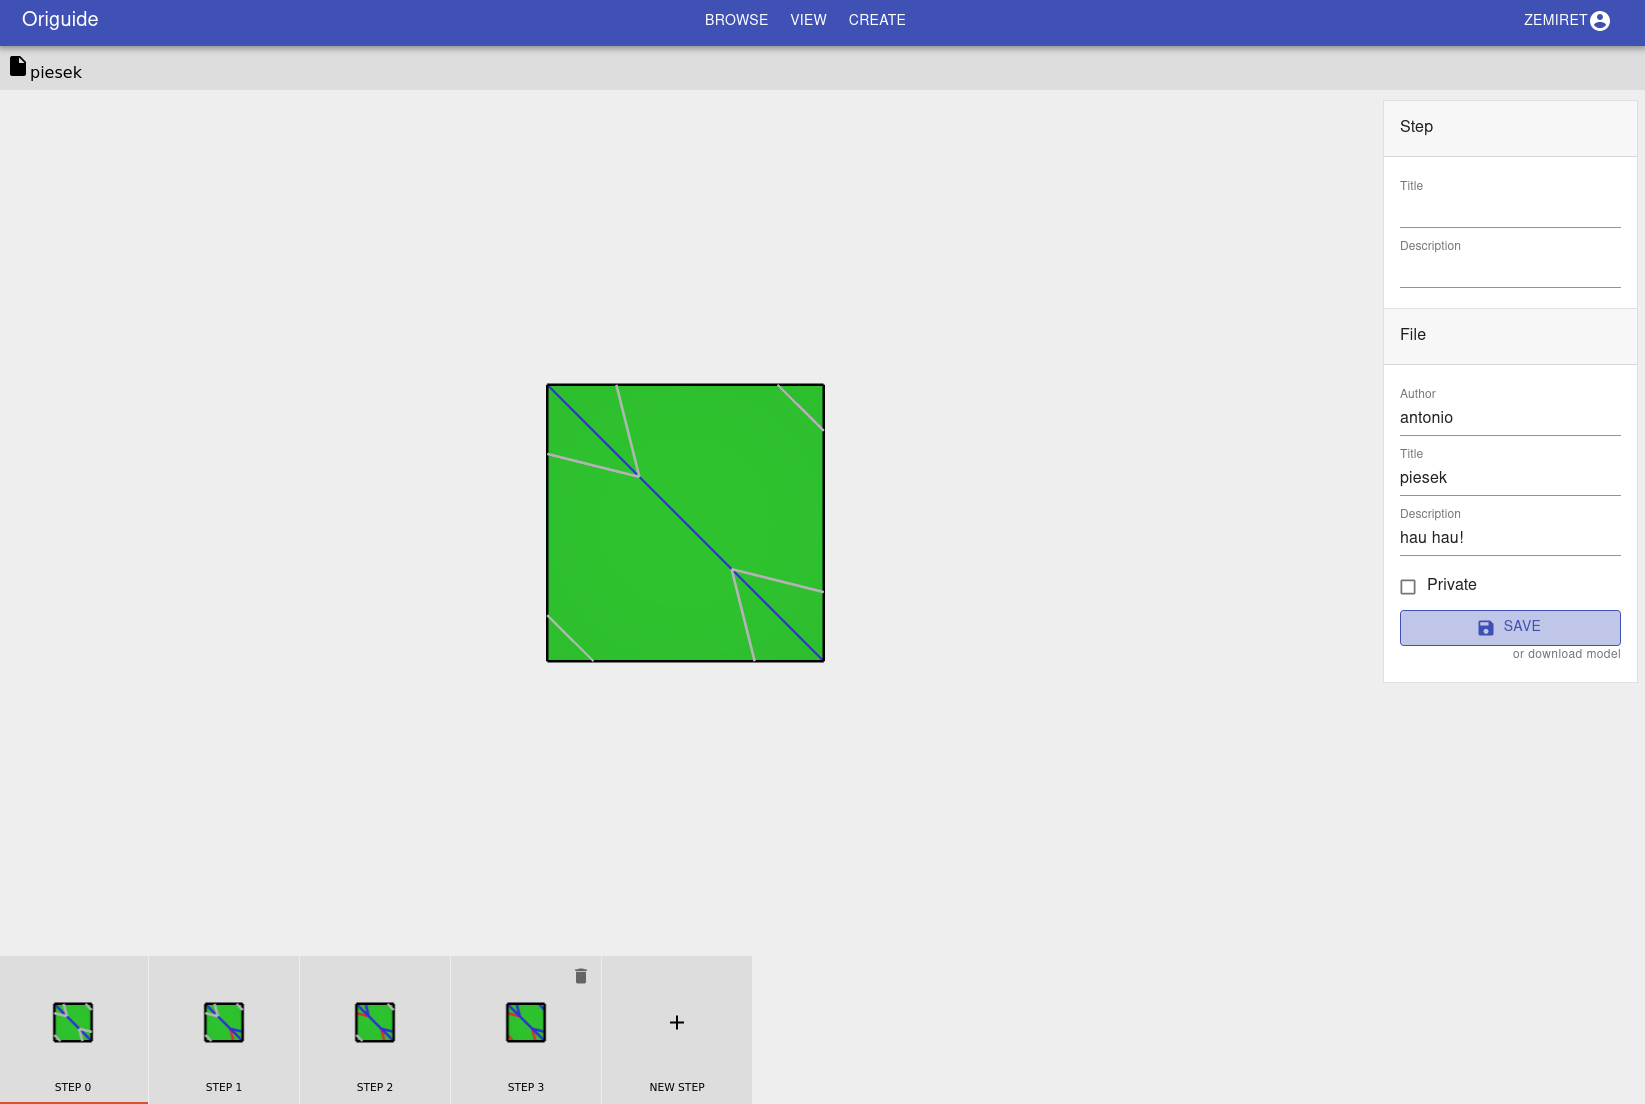
\includegraphics[width=\linewidth]{assets/5-designerSave.png}
\end{frame}
\begin{frame}
  \frametitle{Aspekt społecznościowy}
  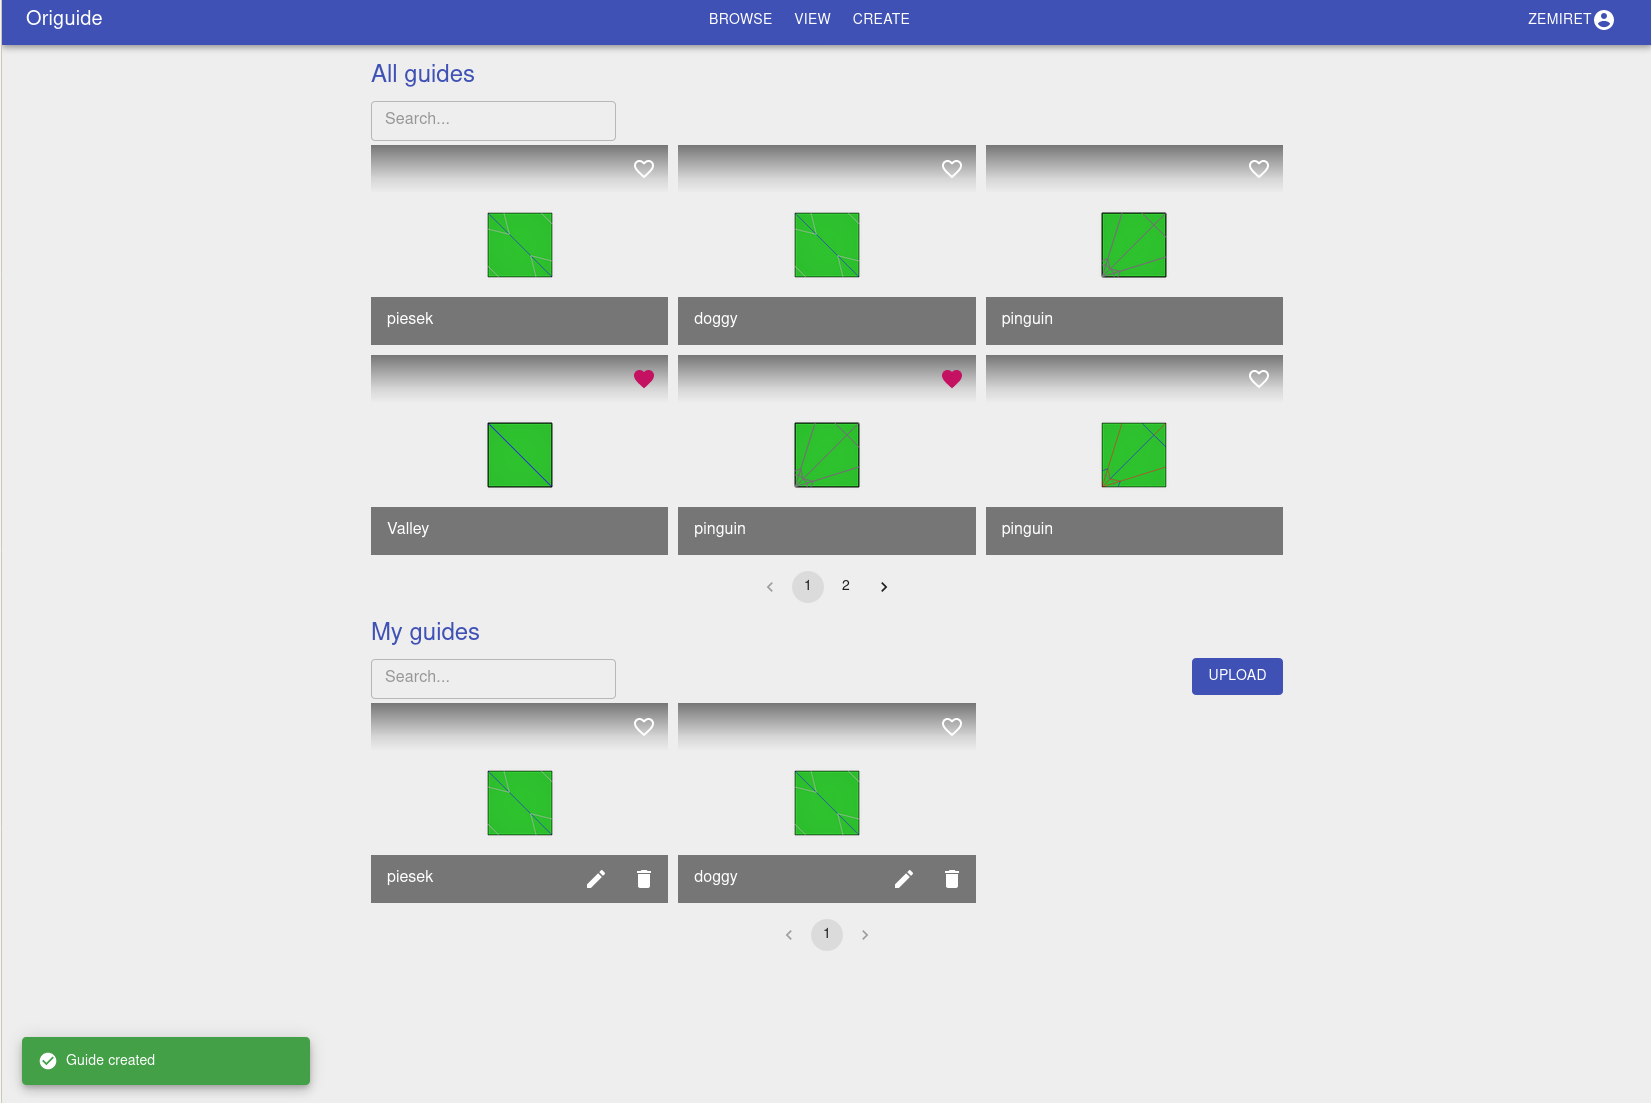
\includegraphics[width=\linewidth]{assets/5-designerBrowser.png}
\end{frame}

\section{Aspekty techniczne}
\begin{frame}
  \frametitle{Architektura}
  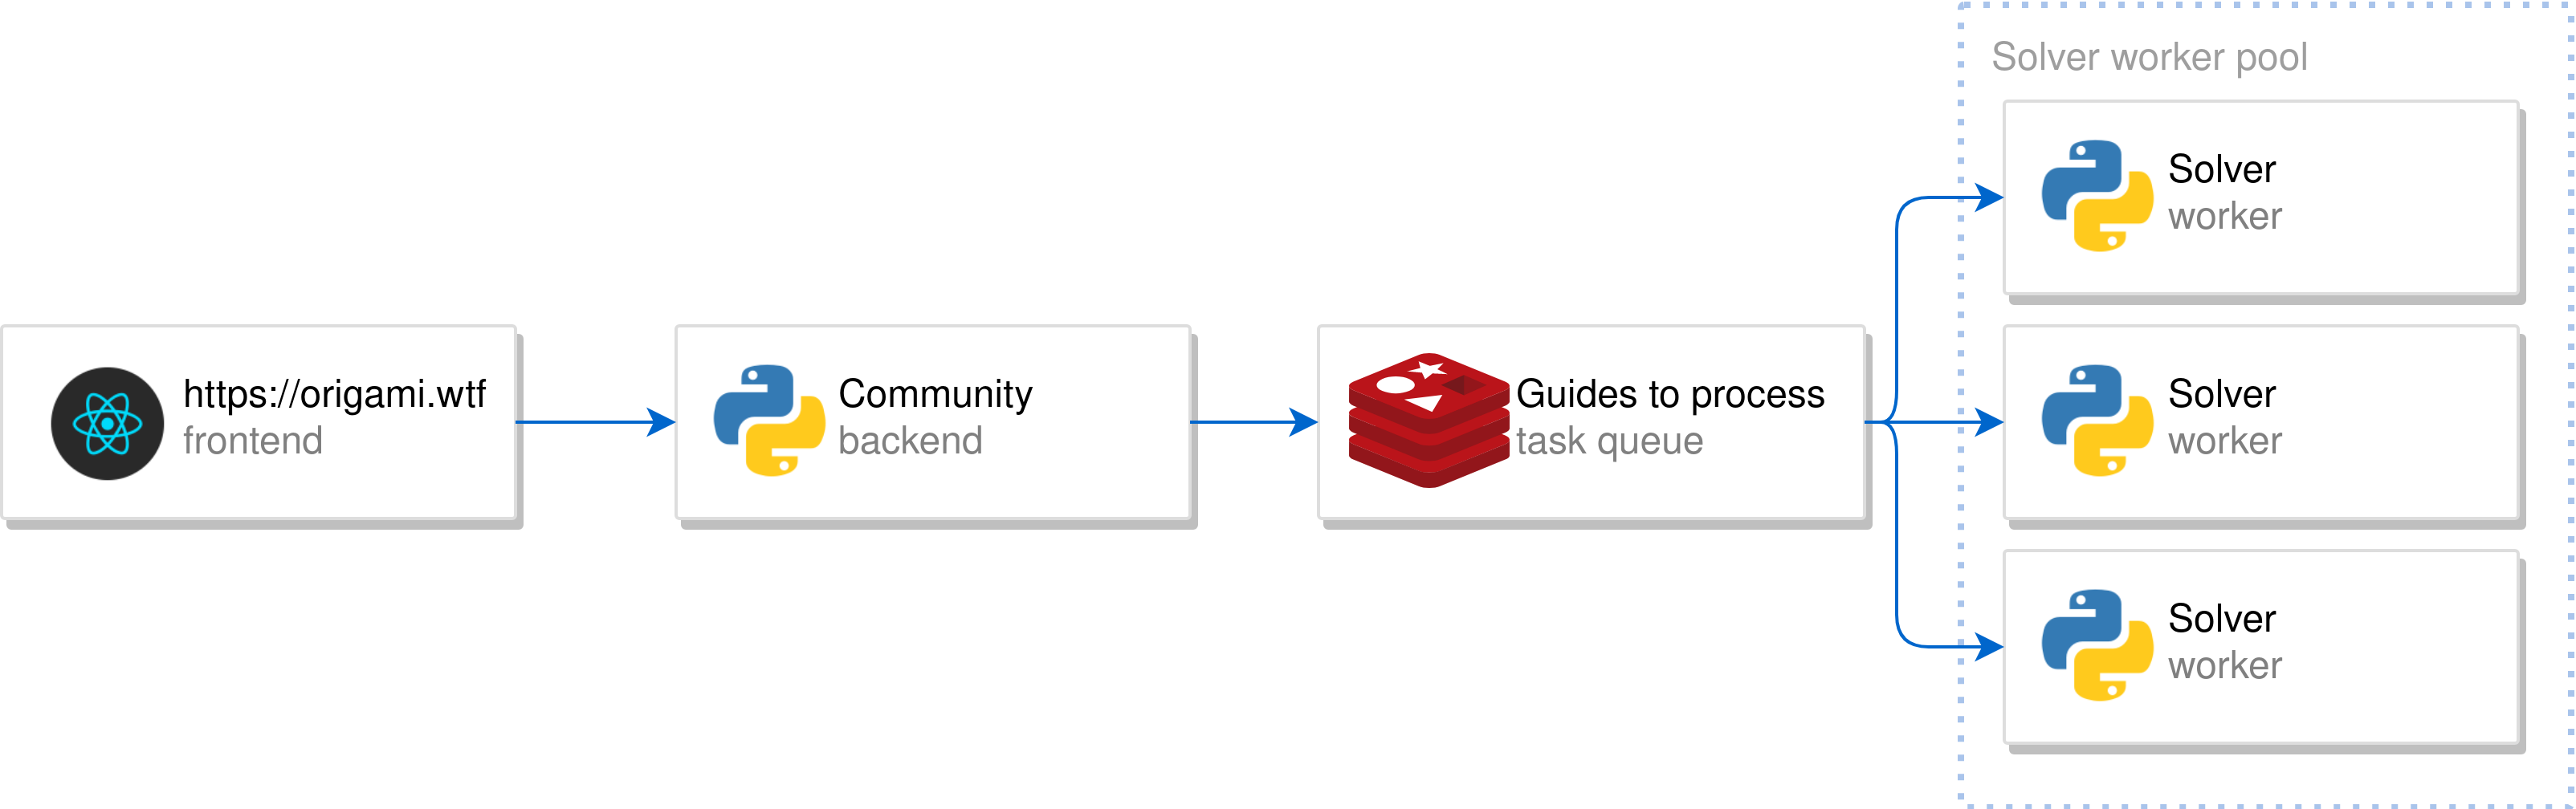
\includegraphics[width=\linewidth]{assets/architecture.png}
\end{frame}
\begin{frame}
  \frametitle{Frontend}
  \centering
  
\includegraphics[width=0.3\linewidth]{assets/react-logo.png}
\end{frame}
\begin{frame}
  \frametitle{Backend - Community}
  \centering
  
\includegraphics[width=0.7\linewidth]{assets/community-stack.png} \\
\end{frame}
\begin{frame}
  \frametitle{Backend - Solver}
  \centering
  
\includegraphics[width=0.5\linewidth]{assets/pypy-logo.png}
\end{frame}

\section{Aspekty implementacyjne}
\begin{frame}
  \frametitle{Aspekty implementacyjne}
  \centering
  	\textbf{Beam} force \\
  	\textbf{Crease} force \\
  	\textbf{Face} force \\
  	\textbf{Damping} force \\
	\vspace{0.5ex}
	
\includegraphics[width=0.03\linewidth]{assets/arrow-down.png}
	\vspace{-2ex}
	\begin{equation*} 
		\pmb{F}_{total} = \sum_{edges} \pmb{F}_{beam} + \sum_{edges} \pmb{F}_{crease} + \sum_{faces}\pmb{F}_{face} + \sum_{edges}\pmb{F}_{damping}
		\vspace{-2ex}
	\end{equation}
	
\includegraphics[width=0.03\linewidth]{assets/arrow-down.png} \\
	Forward Euler integration
\end{frame}

\section{Przebieg prac}
\begin{frame}
  \frametitle{Przebieg prac}
  \centering
	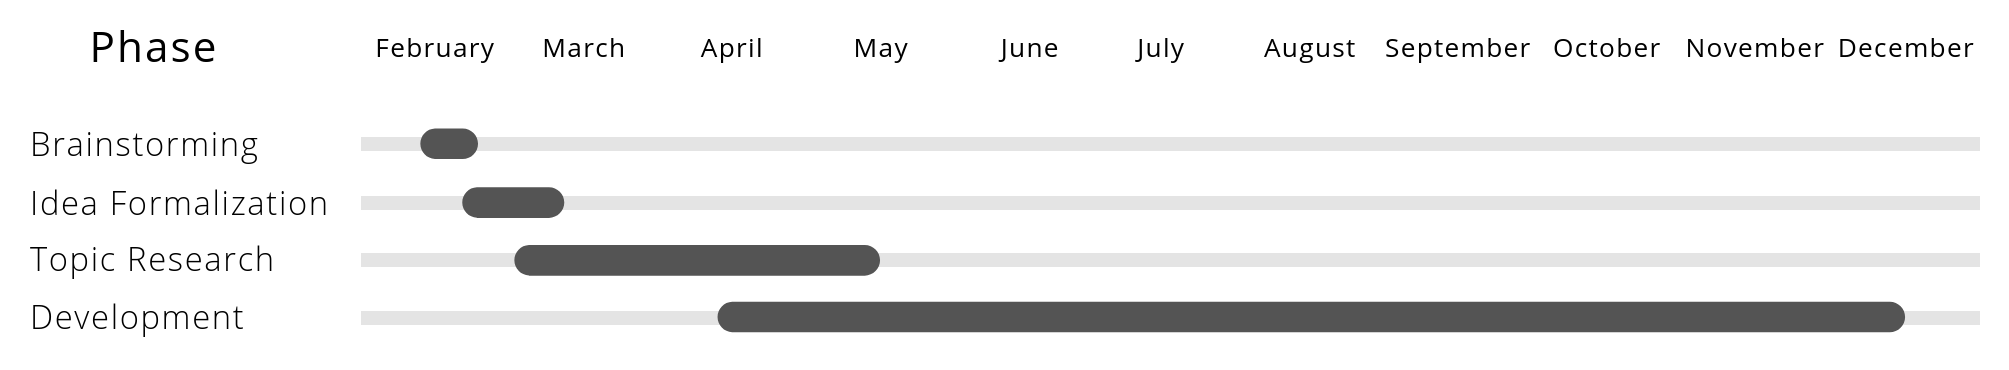
\includegraphics[width=\linewidth]{assets/4-phases.png} \\
\end{frame}

\section{Podział prac}
\begin{frame}
  \frametitle{Podział prac}
  	\hspace{-2ex}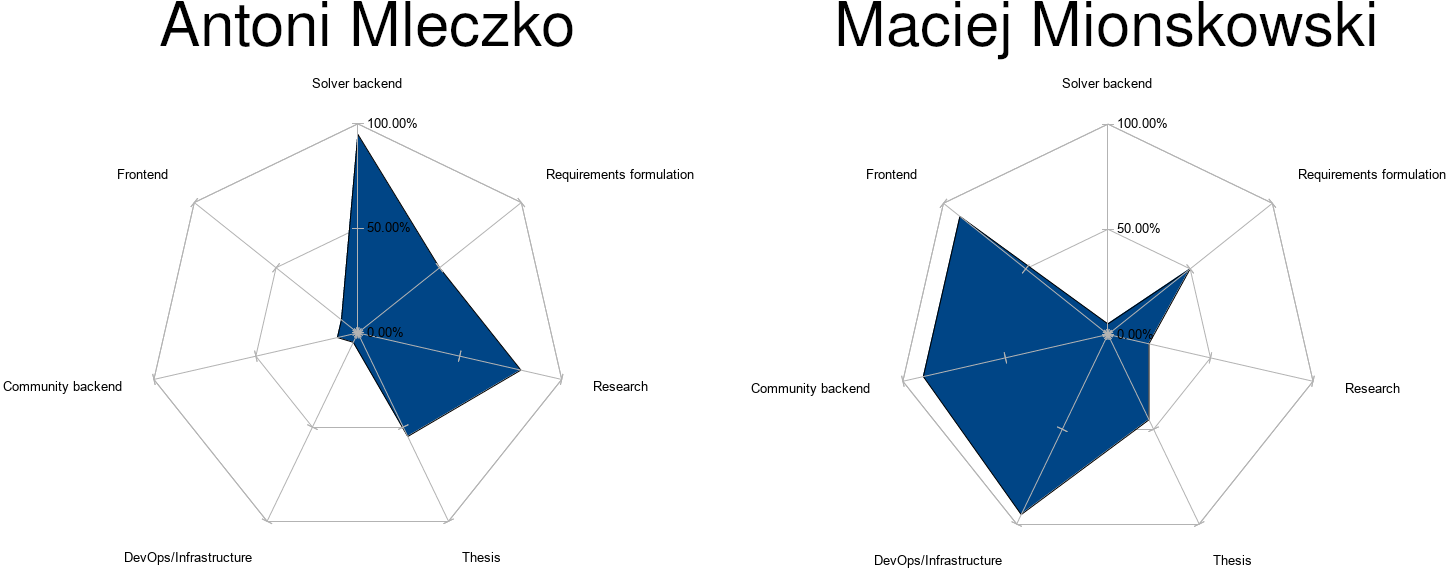
\includegraphics[width=1.04\linewidth]{assets/pres-contribution.png} \\
\end{frame}

\section{Podsumowanie projektu}
\begin{frame}
  \frametitle{Podsumowanie projektu}
  \centering
  \Huge{https://origami.wtf}
\end{frame}

\section{Prezentacja}
\begin{frame}
  \frametitle{Prezentacja}
  \centering
  \Huge{Demo}
\end{frame}



\end{document}
